\section{Arbeitsumgebung und Material}
\label{sec:arbeitsumgebung}
Als Arbeitsort stand uns ein studentischer Arbeitsraum des Fachgebiets Echtzeitsysteme zur Verfügung. Hier wurden die Fahrzeuge aufbewahrt und es waren Arbeitsplätze mit Bildschirmen vorhanden, um die Autos oder eigene Laptops anzuschließen. 
\newline
Die Testfahrten fanden jedoch meist in den Fluren statt. Hier konnten die langen Wände zur Orientierung genutzt werden und es stand etwas mehr Platz zur Verfügung, als im Arbeitsraum. Auch waren von den Vorjahren bereits Querstreifen auf dem Boden angebracht, beispielsweise vor Kurven oder Kreuzungen. Das autonome Fahren gestaltete sich auf den Fluren interessanter, weil hier der recht hohe Wendekreis der Fahrzeuge nicht so ins Gewicht fiel. Außerdem stellten die Flure naturgemäß schon eine realistische Umgebung mit 90° Kurven, Kreuzungen und Hindernissen dar, die von jeder Gruppe individuell genutzt wurde. So war es praktisch keine Einschränkung, dass wir teilweise zur genaueren Positionsbestimmung eine Wand in messbarer Nähe voraussetzten. Geeignete Hindernisse und Tore, bestehend aus Pappkartons mit \textit{ArUco}-Markern, ließen sich natürlich ebenfalls beliebig aufstellen und somit konnten wir immer unterschiedliche Szenarien kreieren. Diese \textit{ArUco}-Marker sind optisch vergleichbar zu QR-Codes. Zudem besteht hier der Vorteil, dass bereits Bibliotheken existieren, die das Erkennen und Auswerten der Marker implementieren.
%%%%%
\begin{figure}[hp] 
  \centering
     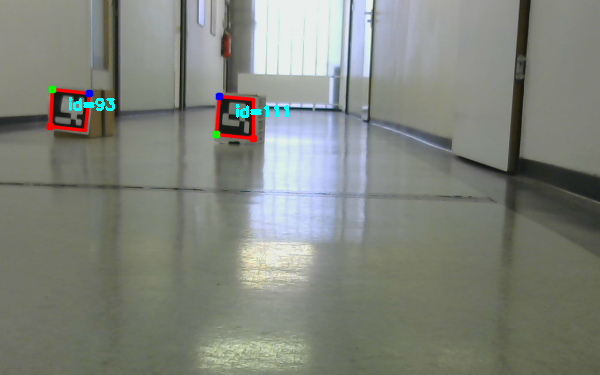
\includegraphics[width=0.9\textwidth]{images/flur.png}
  \caption{\textit{ArUco}-Tor aus Sicht der Kamera}
  \label{fig:ArUco-Tor aus Sicht der Kamera}
\end{figure}
\newline
Dabei können nicht nur die \textit{Id}s der einzelnen Marker ausgelesen werden, sondern auch deren Position im Raum. In der gezeigten Abbildung sehen wir zwei \textit{ArUco}-Marker aus Sicht der Fahrzeugkamera.
